% !TEX TS-program = XeLaTeX
%برای پایان‌نامه ارشد، از خط زیر به جای خط بالا استفاده کنید
\documentclass[Thesis]{thesis}
%اگر نسخه دو رو از پایان‌نامه را می‌خواهید، oneside راحذف کنید
\usepackage[colorlinks=true]{hyperref}

\usepackage{amssymb}
\usepackage[localise]{xepersian}
\usepackage{tikz}
\usetikzlibrary{positioning}

\settextfont[Scale=1,ExternalLocation=fonts/]{XBZar.ttf}
\setdigitfont[ExternalLocation=fonts/]{Yas.ttf}

\localisecommands
\شروع{نوشتار}
\renewcommand{\bibname}{مراجع}

\آرم{\درج‌تصویر{logo}}
\تاریخ{زمستان ۱۳۹۸}
\عنوان{یافتن گلوگاه‌های فرآیندهای کسب و کار با روش‌های یادگیری عمیق}
\نویسنده{سید مرتضی حسینی}
\دانشگاه{دانشگاه شهید بهشتی\\دانشکده علوم و مهندسی کامپیوتر}
\استادراهنما{دکتر صادق علی‌اکبری}
\frontmatter \makethesistitle \pagestyle{empty} \baselineskip1.2\baselineskip

\section*{}
تقدیم به یگانه پناهگاه روز‌های تاریک زندگی، مادر مهربانم.


\شروع{چکیده}{فرآیند‌کاوی LSTM RNN}

پیش بینی فرآیند‌های جاری یک کسب و کار با استفاده از روش های کنترل و پیش بینی مراحل آن با بهره گیری از کاوش داده ها و گزارش های فرآیندهای آن،انجام می‌شود، برای مثال می‌توان به  پیش بینی نتیجه ی این فرآیند، مرحله‌ی بعدی در این فرآیند و یا زمان پایان این فرآیند اشاره کرد. این پیش‌بینی ها و اطلاعات به دست آمده با وجود ماهیت چالشی خود، می‌تواند به ما در تخصیص منابع به هر مرحله کمک شایانی بکند. فاکتور ها و متغیر‌های بسیار زیادی ممکن است در تعیین سرنوشت این فرآیند نقش بازی کنند برای همین فقط استفاده از داده های زمانی فرآیند‌های پیشین به ما کمک چندانی نمی‌کند؛ به همین جهت برای دقیق‌تر کردن پیش‌بینی های خود در این پروژه علاوه بر داده‌های زمانی، از داده‌هایی که به خود  طبیعت آن فرآیند مربوط هستند نیز استفاده می‌کنیم. همچنین برای دقیق‌تر کردن پیش‌بینی های خود از شبکه‌های RNN و به صورت دقیق‌تر شبکه‌های LSTM استفاده می‌کنیم که بتوانیم داده‌های مربوط به زمان را بهتر مدیریت و پیش‌بینی کنیم.

\پایان{چکیده}

    \pagestyle{plain}\pagenumbering{tartibi}\tableofcontents\listoffigures\listoftables

\mainmatter \pagestyle{headings} \baselineskip1.1\baselineskip 
%%%%%%%%%%%%%%%%%%%%%%%%%%%%%%%%%%%%%%%%%%%%%%%%
\فصل{مقدمه}\برچسب{chap:intro}

اساس کار تکنیک‌های مانیتور کردن فرآیندهای کسب و کار ها بر اساس داده ها و مدل‌های استخراج شده از پردازش گزارش‌های فرآیند های قبلی است. بسیاری از تکنیک‌های ارایه شده پیش‌بینی‌های مربوط به: پیش‌بینی فعالیت بعدی، پیش‌بینی مسیر فرآیند در جریان، پیش‌بینی زمان باقی‌مانده، پیش‌بینی تاخیر‌های ممکن یا رسیدن به یک موقعیت خاص می‌باشند. خروجی چنین مدل‌هایی می‌تواند ورودی ارزشمندی برای روند‌های برنامه‌ریزی شرکت‌ها جهت تخصیص منابع باشد.
رویکرد‌های موجود در این زمینه قابلیت گسترش به همه‌ی کسب و کارها را دارا نیستند و فقط روی یک کسب و کار خاص تمرکز دارند. می‌توان گفت که بیشتر الگوریتم‌ها در این حوزه فقط روی دیتاست خود خوب جواب می‌دهند و برای عملکرد خوب روی آن بهینه شده است و ممکن است روی دیتاست دیگری به جواب مناسب نرسد. در بعضی تکنیک‌ها هم چندین روش با هم ترکیب شده است و مدل نیازمند زمان زیادی جهت یادگیری می‌باشد. 
در گزارشات فرآیندهای متفاوت سازمان‌ها، داده‌های متفاوتی قرار دارند، از جمله زمان شروع و پایان این هر مرحله و ترتیب مراحل، اطلاعات فردی که در حال انجام این فرآیند می‌باشد، نام ناظر هر مرحله و ...
داد‌‌ه‌های زمانی قرار داده شده در این گزارشات برای پیش‌بینی زمان اتمام این فرآیند بسیار حائز اهمیت می‌باشد. برای مثال اگر فرض کنیم که یک مرحله‌ای از فرآیند یک روز کاری زمان نیاز دارد تا به اتمام برسد و در بعد از ظهر روز چهارشنبه آغاز می‌شود، با فرض تعطیلی روز‌های پنجشنبه و جمعه به سرعت متوجه می‌شویم که این مرحله روز شنبه به اتمام می‌رسد. برای یک الگوریتمی که قرار است در کامپیوتر اجرا شود این رویه باید به شیوه‌ای مدلسازی شود. در این مثال ساده می‌توان با یک ساختار شرطی ساده مانند if-then-else قبل از انجام پیش‌بینی متوجه این مورد بشویم و به زمان پیش‌بینی خود دو روز اضافه کنیم اما این روش به سختی قابل گسترش است و به روش‌های کلی‌تری نیاز داریم.
همچنین گفتیم که علاوه‌بر داده‌های زمانی، داده‌های دیگری ممکن است در اختیار ما قرار بگیرد. برای مثال اگر فرآیند ثبت‌نام ترم دانشجو در دانشگاه را در نظر بگیریم، سیستم ثبت‌نام علاوه بر زمان هر رخداد (مانند: ورود به سیستم، ثبت درخواست دریافت درس و ...) داده‌های دیگری هم به ما می‌دهد. ازین داده‌ها می‌توان به معدل فرد، شهریه‌ی قابل پرداخت و سن اشاره کرد. حدس اولیه‌ی ما این است که از این داده‌ها که علاوه بر داده‌های زمانی تهیه شده می‌توان استفاده کرد تا پیش‌بینی‌های دقیق‌تری برای فرآیند ها انجام شود.ولی باید بتوانیم این داده‌ای اضافی را به صورت خوبی برای کامپیوتر و مدل یادگیری عمیق خود مدل کنیم تا بهترین بهره را از آن‌ها ببریم. 
دیدیم که شبکه‌های RNN و همچنین LSTM می‌توانند نتایج بسیار خوبی روی داده‌های دنباله‌ای مانند زبان‌های طبیعی یا گفتار به ما بدهند. از آنجایی که جنس مساله‌ی ما به خوبی می‌تواند به صورت  دنباله‌ای مدل شود، پس چنین شبکه‌های می‌توانند نتایج بسیار خوبی روی این مساله برای ما پدید آورند.
در این پروژه قصد داریم با استفاده از شبکه‌های LSTM بتوانیم در فرآیند جاری، رویداد بعدی و زمان رخداد آن را پیش‌بینی کنیم. همچنین کل زمان این فرآیند را پیش‌بینی کنیم.

\قسمت{حوزه فرآیندکاوی}
فرآیندکاوی ، خانواده ای از تکنیک ها در زمینه مدیریت فرآیند است که از تجزیه و تحلیل فرآیندهای تجاری بر اساس گزارش ارائه داده شده از روند فرآیند‌ها انجام می‌شود. در طی فرآیندکاوی، الگوریتم های تخصصی داده کاوی برای شناسایی الگوها و جزئیات موجود در روی داده های ثبت شده توسط سیستم اطلاعاتی، اعمال می شوند. هدف از استخراج فرآیند بهبود بهره وری و درک فرایندها است. در ادبیات دانشگاهی اصطلاح خودکار کشف فرآیند کسب و کار به معنای جزئی‌تری به کار می رود تا بطور خاص به تکنیک‌هایی که به عنوان ورودی یک گزارش فرآیند دریافت می‌کنند و یک مدل جهت برداشت اطلاعات از فرآیند به عنوان خروجی تحویل می‌دهند، اشاره کند. اصطلاح Procing Mining در یک محیط گسترده تر مورد استفاده قرار می گیرد تا نه تنها به تکنیک های کشف مدل های فرآیند، بلکه به روش‌های درستی سنجی و تجزیه و تحلیل فرآیند‌ها، اشاره کند.


\قسمت{کاربرد‌ها}
فرآیندکاوی می تواند برای بهبود فرآیند و نظارت بر رفتار مشتریان استفاده شود. یک فرایند تجاری زنجیره‌ای از فعالیت هایی است که برای رسیدن به یک هدف به یکدیگر وصل می شوند. گاهی ممکن است بر خلاف اسناد موجود، بین مراحل مختلف یک فرآیند فاصله چشمگیری وجود داشته باشد. با استفاده از فرآیندکاوی، می توانیم اجرای واقعی فرآیند را بررسی کنیم و بتوانیم ناکارآمدی، گلوگاه‌ها و انحرافات از یک فرآیند را تشخیص دهیم. پس از شناسایی و اولویت بندی مراحل قابل بهبود، می‌توان اقدامات لازم در جهت بهبود روند فرآیند را انجام داد. فرآیندکاوی می‌تواند با یک تحلیل بر اساس اطلاعات در دسترس، برای تشخیص مناطق بهبود مورد استفاده قرار گیرد.
فرآیندکاوی به صورت مداوم قابل استفاده است. پس از حل یک گلوگاه، تمرکز به سمت رفع ناکارآمدی بعدی تغییر می کند. استخراج فرآیند نباید به عنوان یک پروژه کوتاه مدت، بلکه یک تکنیک مداوم بهبود فرآیند تلقی شود.
فرآیندکاوی فقط برای تجزیه و تحلیل فرآیندها پس از اتمام آن‌ها مورد استفاده قرار نمی گیرد. همچنین می توان از آن برای پیش بینی اجرای یک فرآیند(به عنوان مثال زمان باقیمانده و احتمال موفقیت) استفاده کرد و اقدامات مناسب را پیشنهاد کرد.

\قسمت{تعریف مساله}

در این پایان‌نامه قصد داریم که با ورودی گرفتن گزارشات فرآیند‌ها به صورت یک دنباله از مراحل مختلف، بتوانیم گلوگاه فرآیند‌های جاری را پیش‌بینی کنیم. منظور از گلوگاه مرحله‌ای است که بیشترین مدت زمان انجام را داراست. برای حل این مساله ابتدا پیش‌بینی می‌کنیم که فرآیند‌جاری تا پایین چه مراحلی را طی می‌کند و هر مرحله را در چه زمانی انجام می‌دهد. سپس بیشترین فاصله‌ی بین دو مرحله را به عنوان مدت زمان گلوگاه و مرحله مربوطه را به عنوان گلوگاه معرفی می‌کنیم.


\قسمت{کاربرد یافتن گلوگاه‌ها}

مساله‌ی تخصیص منابع در یک کسب و کار مساله‌ی مهمی در جهت مدیریت دارایی و نیرو‌های آن کسب و کار می‌باشد. اگر در فرآیند‌های یک کسب و کار مرحله‌ای بیشترین زمان را به خود اختصاص دهد می‌توان گفت که آن مرحله بیشترین هزینه را به مجموعه تحمیل می‌کند. با یافتن و بهبود این گلوگاه‌ها می‌توان بسیاری از هزینه‌ها را کاهش داد. همچنین با پیش‌بینی گلوگاه روند جاری می‌توان به مشتری کمک کرد تا از آینده‌ی درخواست خود آگاه شود و با توجه به زمان مورد نیاز برای هر بخش بتواند به خوبی برنامه ریزی نماید.



\فصل{کار‌های انجام شده و چالش های پیش‌رو}

در زمینه‌ی فرآیندکاوی در حال حاضر مقالات زیادی منتشر شده است و کار‌های زیادی صورت گرفته است. اولین تحقیقاتی که در این زمینه صورت گرفته به زمینه ای به نام  "پایش فرآیند‌های کسب و کار" 
\پانویس{Business Activity Monitoring}
\cite{datawarehouse}
برمی‌گردد. در \cite{regression} با کمک رگرسیون خطی، مدلی توسعه داده شده است که از تمام داده‌های گزارشات استفاده می‌کند و زمان باقی‌مانده برای اتمام یک فرآیند را به دست می‌آورد. در \cite{next} از گزارشات استفاده می‌کند و می‌تواند محتمل‌ترین گام پیش رو را پیش‌بینی کند. نرم‌افزار TIBCO یکی از اولین ابزار‌های تجاری معرفی شده در این زمینه است. این نرم‌افزار با استفاده از داده‌هایی که اپراتور آن به صورت دستی به آن می‌دهد مانند مسیر‌های بین ف‌ها یا مدت زمانی که انتظار می‌رود تا هر مرحله به طول انجامد، می‌تواند مرحله‌ی بعدی و زمان هر مرحله را پیش‌بینی کند. در \cite{tree} از یک درخت تصمیم گیری استفاده می‌شود که بر روی دیتای جمع آوری شده است، ساخته می‌شود و از این درخت برای حدس زدن مرحله‌ی بعدی استفاده می‌شود. 
به تازگی روش‌هایی مطرح شدند که از یادگیری عمق استفاده می‌کنند. در \cite{deep1} از یک شبکه عصبی استفاده می‌شود که از دو لایه‌ی بازگشتی با ساختار ساده‌ی LSTM استفاده شده است. در \cite{cluster1} یک روش دو مرحله‌ای اتخاذ شده است. در مرحله‌ی نخست داده‌ها به صورت بدون نظارت \پانویس{Unsupervised Learning} خوشه‌بندی می‌شوند و در مرحله‌ی بعد هر خوشه به صورت جداگانه با استفاده از مدلی بر اساس درخت‌های تصادفی \پانویس{Random Forrests} پردازش می‌شود. نزدیکترین اثر مرتبط با کاری که در این پایان‌نامه ارائه شده است مقاله \cite{process} است ، جایی که نویسندگان یادگیری چند وظیفه ای را پیشنهاد می کنند که مدل آن بر اساس یک شبکه‌ی LSTM طراحی شده است. مدل، فعالیت بعدی و مدت زمان آن را پیش بینی می کند و سپس ، مدل قادر به پیش بینی ادامه‌ی روند می‌باشد که از طریق تکرار پیش‌بینی کردن مرحله‌ی بعد به دست می‌آید. این رویکرد هنگامی که مراحل تکراری زیادی وجود داشته باشد عملکرد بدی از خود نشان خواهد داد.





%%%%%%%%%%%%%%%%%%%%%%%%
\فصل{روش پیاده‌سازی شده}\برچسب{chap:rnn}

در این بخش ابتدا به توصیف شبکه‌ی عصبی استفاده‌شده می‌پردازیم، سپس ایده‌ی کلی پیاده‌سازی شده را بیان می‌کنیم و سپس به مقایسه پیاده‌سازی‌های مختلف می‌پردازیم.

\قسمت{شبکه‌های هم‌زمان}\برچسب{chap:rnn}
انسان‌ها هر موقع که در حال تفکر هستند، پیش‌فرض‌های ذهنی‌ای دارند که معمولا به آن‌ها در پیش‌برد فرآیند تفکر کمک می‌کند. وقتی شما این پایان‌نامه را مطالعه می‌کنید هر کلمه را با توجه با کلمه‌ی قبل پردازش می‌کنید. در واقع تفکر انسان نوعی ذخیره‌سازی در خود دارد. 
شبکه‌های عصبی معمولی این قابلیت را ندارند. مثلا فرض کنید بخواهیم که اتفاقات هر فریم یک فیلم را طبقه‌بندی ‌(Classify) کنیم. شبکه‌های عصبی معمولی نمی‌توانند این طبقه‌بندی را بر اساس داده‌هایی که از فریم‌های گذشته به دست آورده‌اند انجام دهند.
شبکه‌های عصبی بازگشتی (Recurrent) برای حل همین مشکل ساخته شده‌اند. شبکه‌هایی که با داشتن حلقه‌ می‌توانند اطلاعات را در خود نگه‌داری کنند.

\begin{figure}[h]
\centering
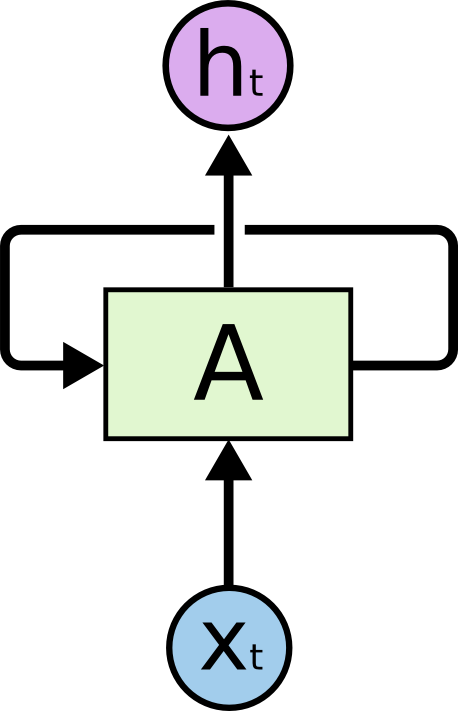
\includegraphics[scale=0.5]{RNN-rolled}
\caption{شبکه‌های هم‌زمان دارای دور می‌باشند.}
\label{fig:rolled}
\end{figure}
شکل \ref{fig:rolled} که یک قسمت از یک شبکه عصبی می‌باشد، A یک ورودی مانند $x_t$ دریافت می‌کند و یک مقدار مانند  $h_t$ خروجی میدهد. یک حلقه این قابلیت را فراهم ‌می‌کند که داده و اطلاعات از یک مرحله به مرحله‌ی بعدی منتقل شود.
یک شبکه‌ی RNN در واقع چند کپی از یک شبکه هست که هر کدام از این کپی‌ها پیامی را به شبکه‌ی بعدی خود منتقل می‌کنند. اگر حلقه را باز کنیم با زنجیره‌ای مانند شکل \ref{fig:unrolled}  روبرو خواهیم شد. همچنین مقادیر داخل شبکه در \ref{fig:states} نشان داده شده است.
\begin{figure}[h]
\centering
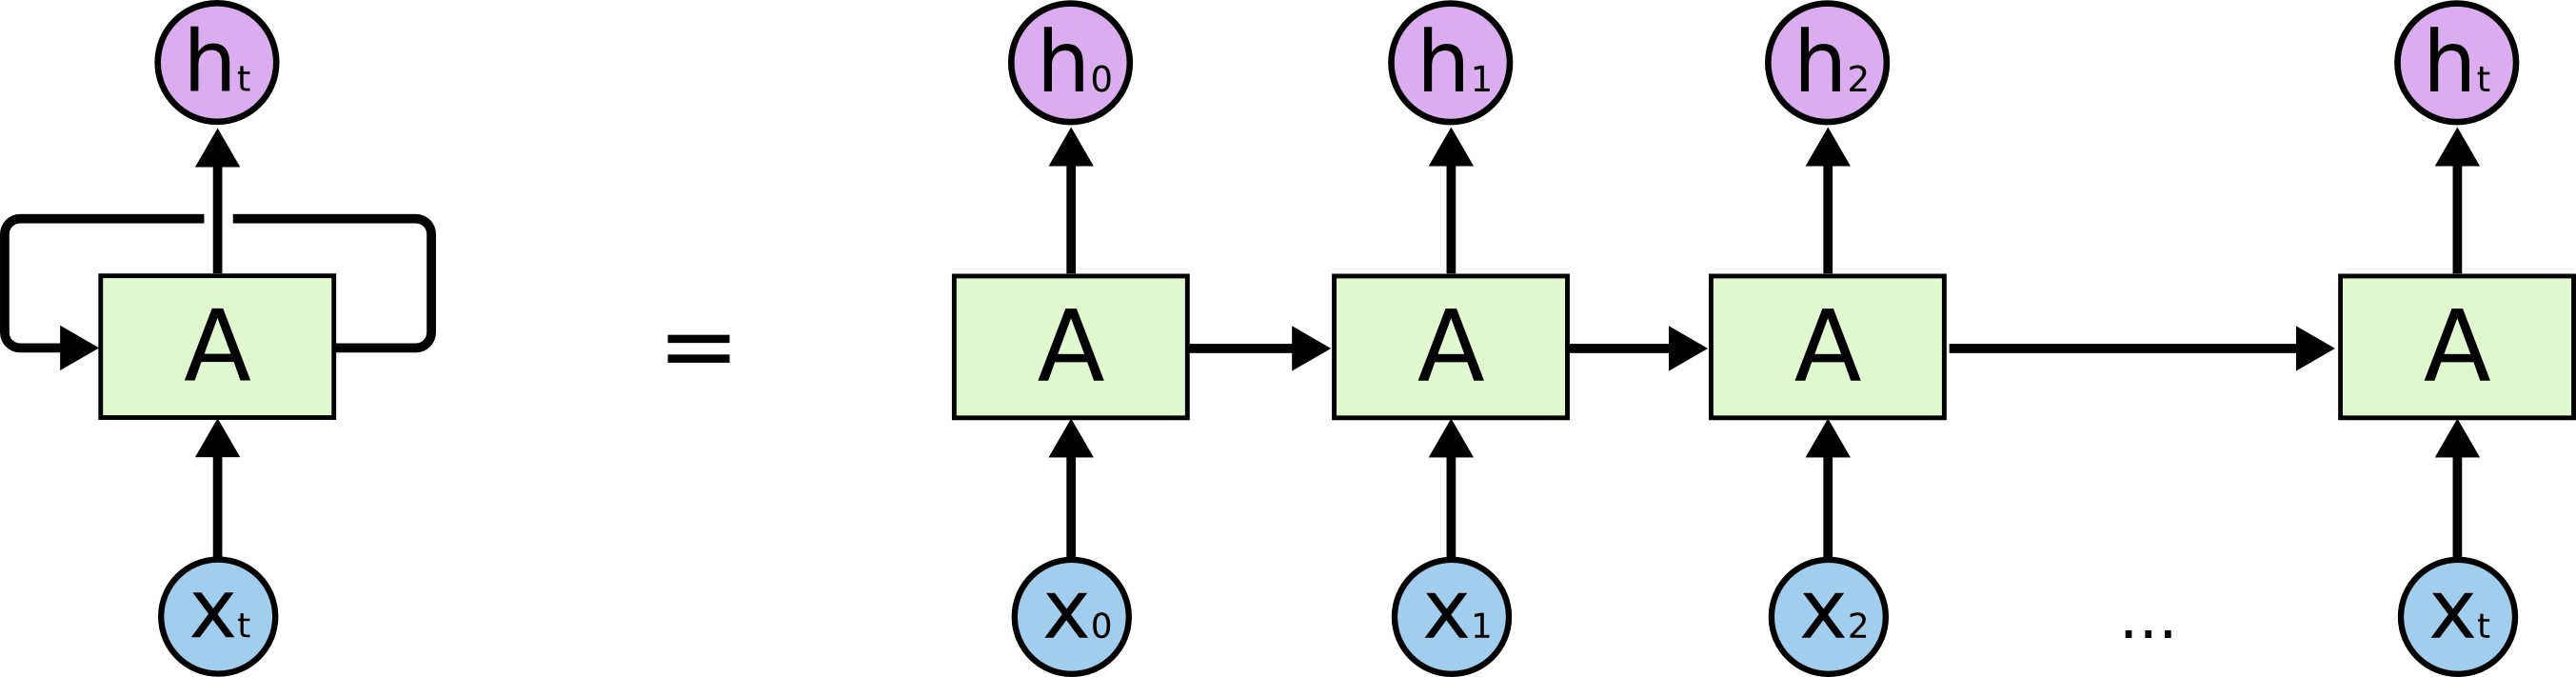
\includegraphics[scale=0.35]{RNN-unrolled}
\caption{نمایش دور‌های شبکه به صورت باز شده.}
\label{fig:unrolled}
\end{figure}
میتوان به صورت کلی شبکه‌های بازگشتی را با فرمول‌های \ref{eq:rnn1} و \ref{eq:rnn2} مدل کرد


\begin{equation}
a^{< t >}=g_1(W_{aa}a^{< t-1 >}+W_{ax}x^{< t >}+b_a)\label{eq:rnn1}
\end{equation}

\begin{equation}
y^{< t >}=g_2(W_{ya}a^{< t >}+b_y)\label{eq:rnn2}
\end{equation}
که $W_{ax}, W_{aa}, W_{ya}, b_a, b_y$ ضرایبی هستند که به صورت موقتی بین حالات در اشتراک هستند و $g_1, g_2 $تابع‌های فعال سازی هستند.

به صورت کلی می‌توان گفت که شبکه‌های هم‌زمان برای ما مزایای زیر را خواهد داشت:
\begin{itemize}
  \item می‌توانند ورودی به هر طولی را پردازش نمایند
  \item اندازه‌ی مدل با افزایش سایز مساله بزرگ نمی‌شود.
\item ضرایب در زمان‌های متفاوت یکسانند.
\item محاسبات توانایی این را پیدا می‌کنند که از داده‌های قبل از خود استفاده کنند.
\end{itemize}
را خواهد داشت.
و البته مشکلات :

\begin{itemize}
\item محاسبات کند می‌شوند.
\item در دسترسی به داده‌های خیلی قدیمی مشکل دارند.
\item داده‌های آینده را برای حالت جاری در نظر نمیگیرند.
\end{itemize}

را هم دارا هستند.
\begin{figure}[h]
\centering
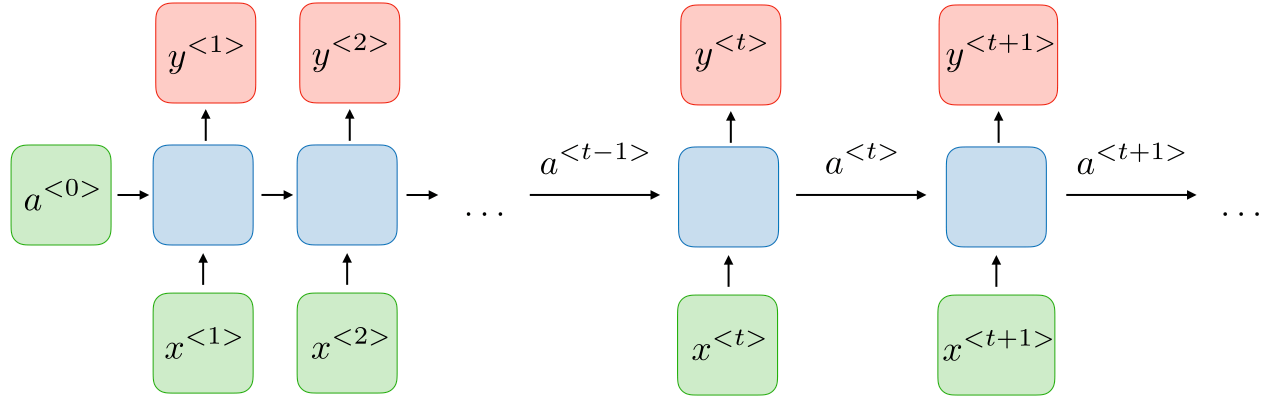
\includegraphics[scale=0.35]{arch-rnn}
\caption{حالات درون شبکه.}
\label{fig:states}
\end{figure}

\قسمت{مشکل حافظه کوتاه مدت}
کار‌هایی را در نظر بگیرید که در آن‌ها مدل ما نیاز دارد که به اطلاعات پیشین خود برای انجام کار دسترسی داشته باشد. برای مثال سناریویی را در نظر بگیرید که مدل ما کلمه‌ی بعدی یک جمله را پیش‌بینی می‌کند. در جمله‌ی "ابر ها در آسمان هستند" برای پیش‌بینی کلمه‌ی "آسمان" به جملات قبل این جمله نیاز نداریم و به راحتی می‌توان "آسمان" را پیش بینی کرد. در چنین مثال‌هایی که فاصله‌ی میان داده‌های مورد نیاز کم است، شبکه‌های هم‌زمان می‌توانند طوری آموزش ببینند که به راحتی از داده‌های گذشته استفاده کنند. این موضوع در شکل \ref{fig:rnngood} نمایش داده شده است. 
\begin{figure}[h]
\centering
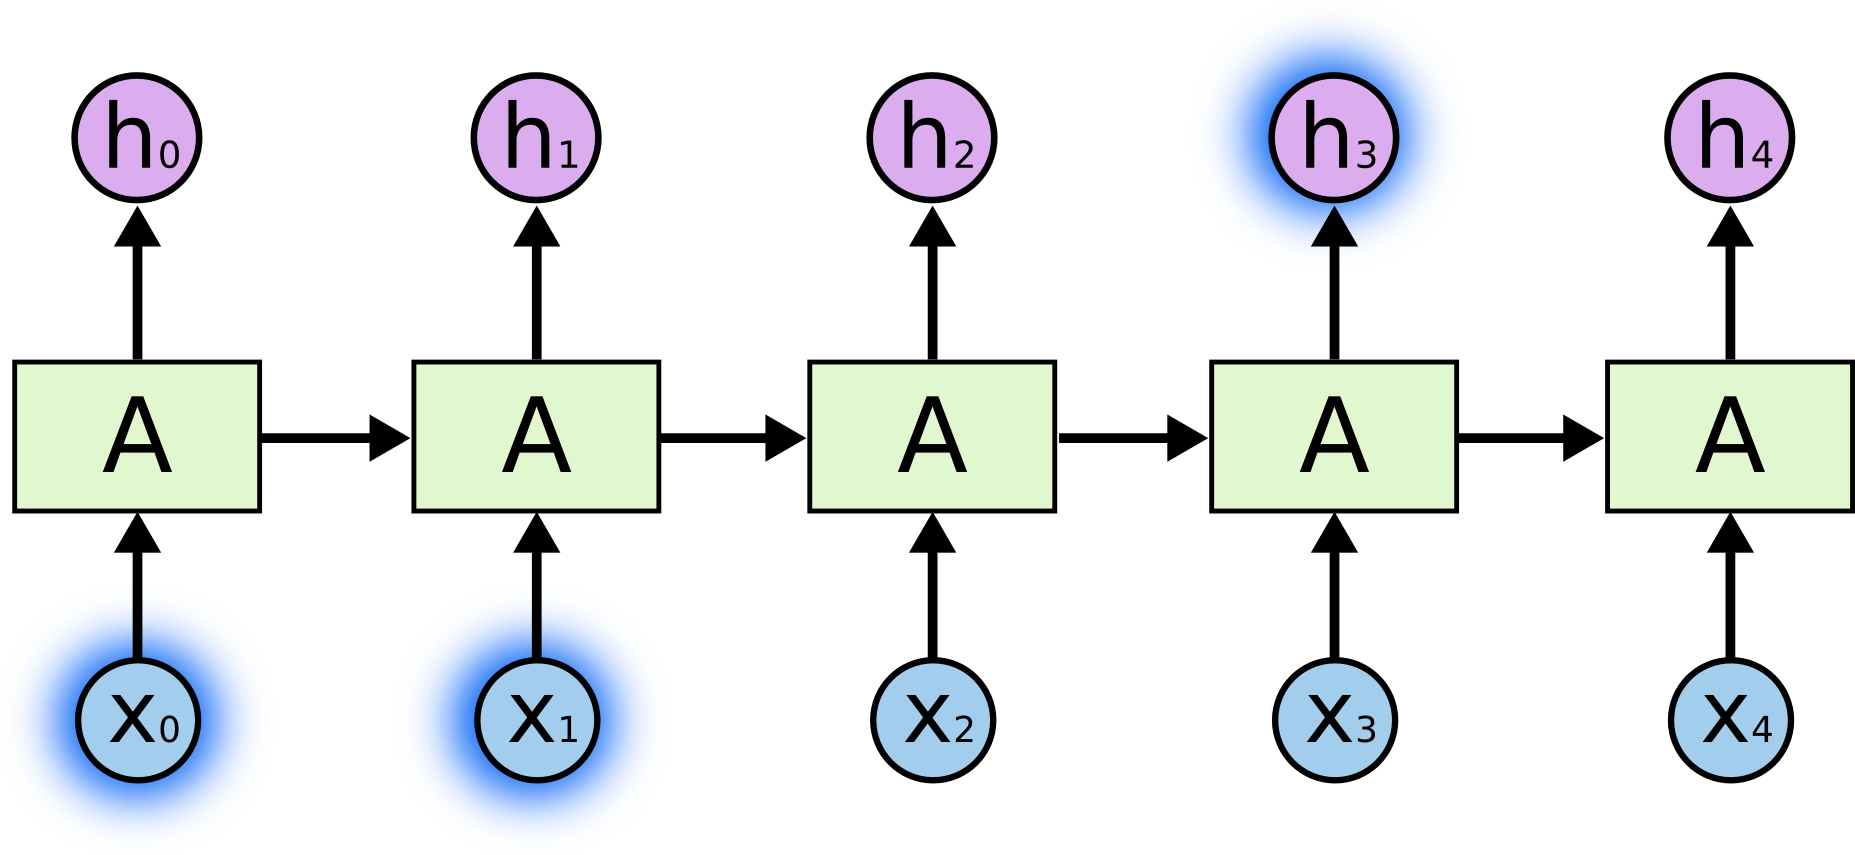
\includegraphics[scale=0.35]{RNN-isgood}
\caption{شبکه راحت‌تر می‌تواند از داده‌های کمتر قدیمی بهره ببرد.}
\label{fig:rnngood}
\end{figure}
اما مواردی نیز هستند که به داده‌های بسیار قدیمی‌تر برای انجام پیش‌بینی نیاز داریم. برای مثال در جمله‌ی "من در ایران زاده شده‌ام. ..... زبان مادری من فارسی است" برای پیش‌بینی کلمه‌ی "فارسی" ممکن است به داده‌های خیلی قدیمی ای نیاز پیدا کنیم. البته در تئوری ممکن است که با بازی کردن با وزن‌های شبکه خود بتوانیم از داده‌های خیلی قدیمی‌تر خود استفاده کنیم اما در عمل به دلیل وجود مشکل مشتق‌های انفجاری و محو شونده این کار بسیار سخت می‌شود. این موضوع در شکل \ref{fig:rnnbad} نمایش داده شده است.


\begin{figure}[h]
\centering
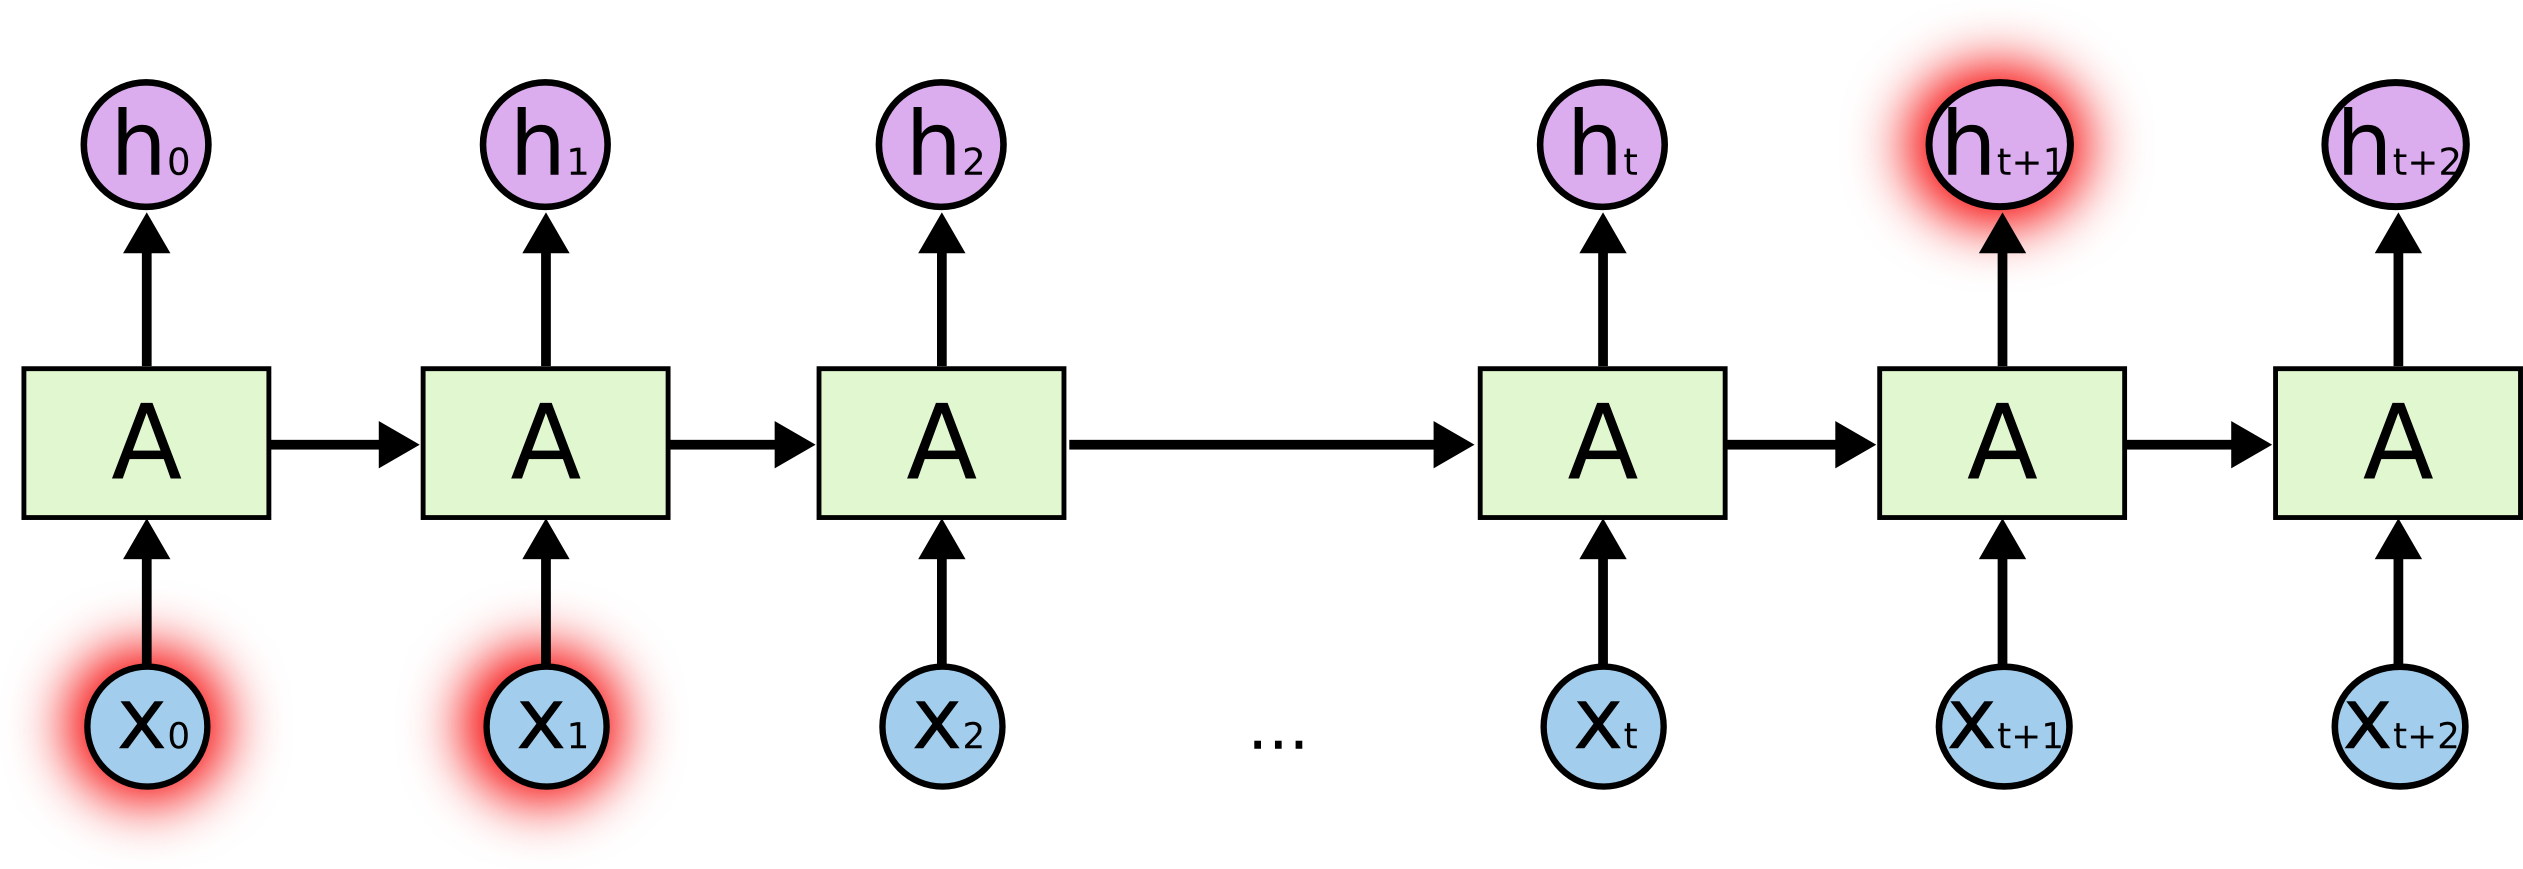
\includegraphics[scale=0.35]{RNN-isbad}
\caption{با زیاد شدن فاصله شبکه بدتر کار خواهدکرد.}
\label{fig:rnnbad}
\end{figure}
\قسمت{مشتق‌های انفجاری و محو‌شونده}
مشتق‌های انفجاری و محو‌شونده پدیده‌هایی هستند که در شبکه‌های هم‌زمان ممکن است به آن‌ها بر بخوریم. علت آن هم این است که با زیاد شدن لایه‌های شبکه، مقدار مشتق ممکن است نمایی بزرگ یا کوچک شود برای همین تاثیر آن در لایه‌های پیشین نادرست خواهد شد.
برای حل این مشکل باید از شبکه های هم‌زمان از نوع حافظه‌ی طولانی مدت استفاده کنیم.

\قسمت{شبکه‌های حافظه طولانی مدت}\برچسب{chap:lstm}

شبکه‌‌های حافظه طولانی مدت نوع خاصی از شبکه‌های همزمان هستند که می‌توانند وابستگی‌های طولانی مدت را یاد بگیرند. این شبکه‌ها برای یادگیری وابستگی‌های طولانی مدت طراحی شدند و این خاصیت طبیعی آنان می‌باشد و نیاز به سختی در وزن‌دهی یا بالابردن مدت زمان یادگیری ندارند.
تمام شبکه‌های هم‌زمان یک ماژول تکرار شونده گاهی به سادگی یک $tanh$ ساده مانند شکل \ref{fig:rnntanh} را دارا هستند. در شبکه‌های LSTM این ساختار تکرار شونده ساختمان متفاوتی دارد. به جای یک لایه شبکه‌ی عصبی، چهار لایه مانند شکل \ref{fig:lstmf} داریم که به صورت خاصی با هم در تعامل هستند.
 
\begin{figure}[h]
\centering
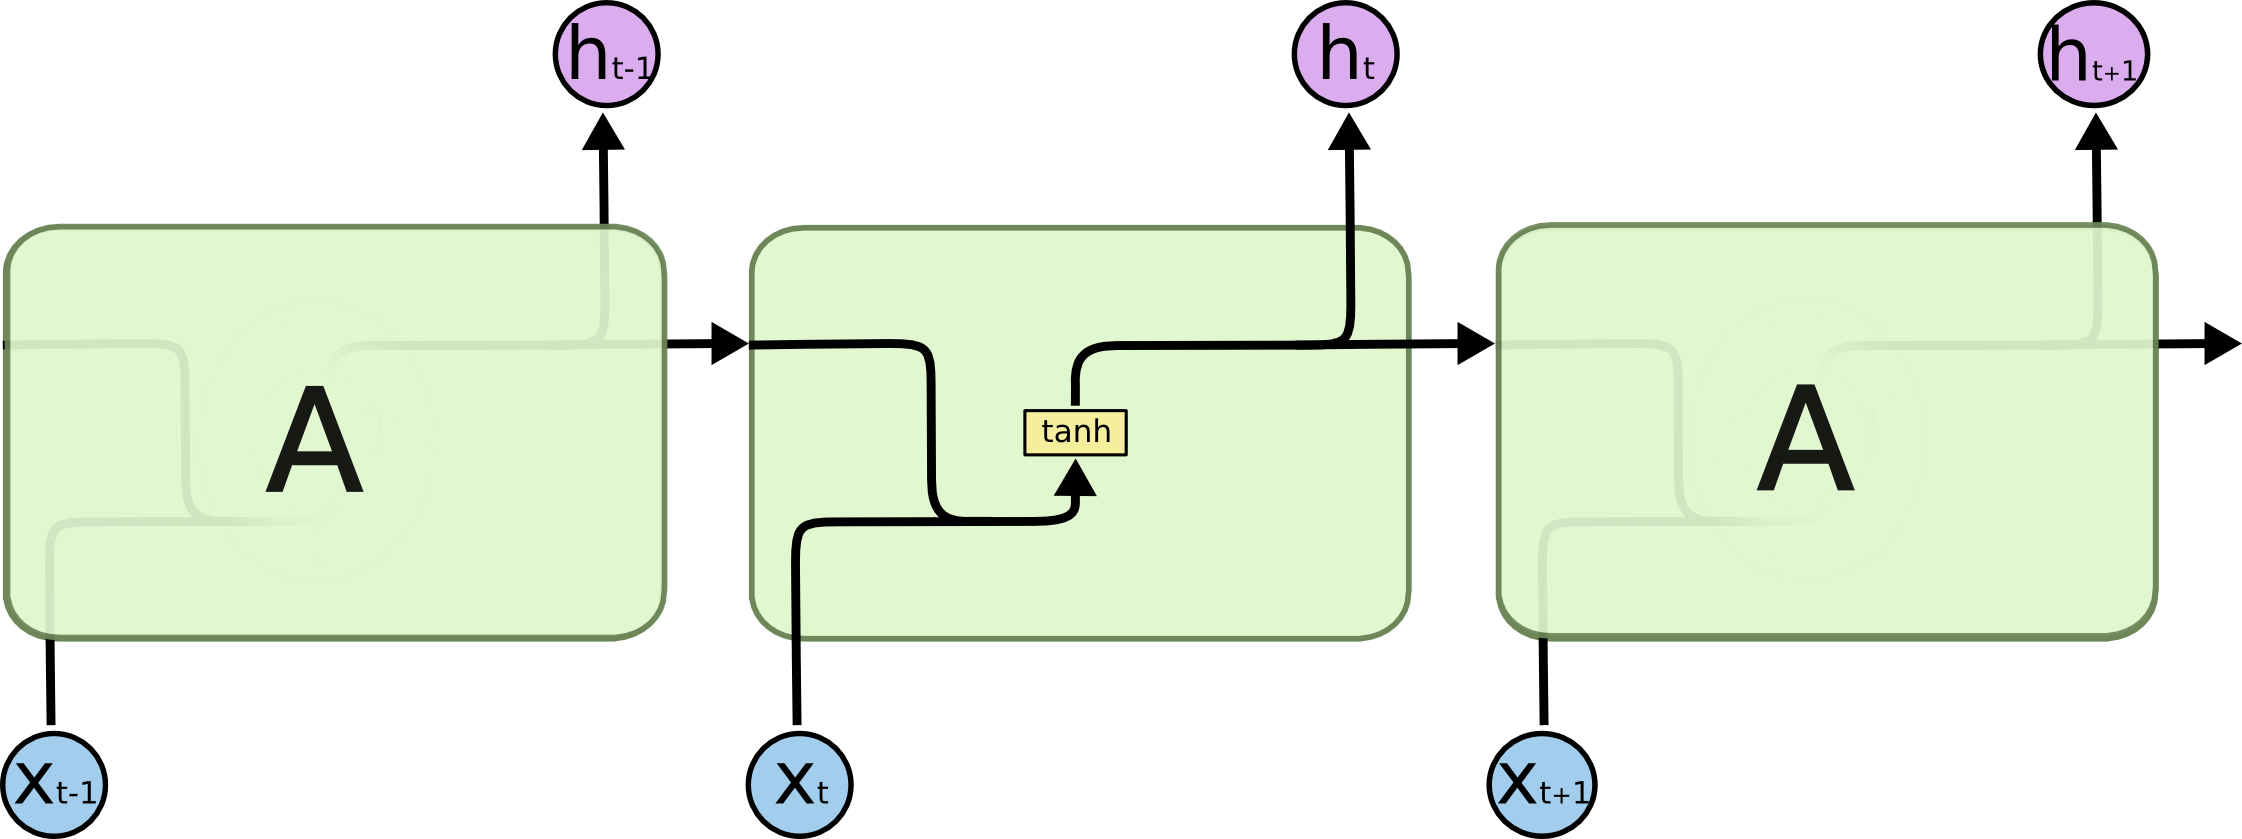
\includegraphics[scale=0.35]{LSTM3-SimpleRNN.png}
\caption{ساختار شبکه‌های ساده‌ی هم‌زمان}
\label{fig:rnntanh}
\end{figure}
\begin{figure}[h]
\centering
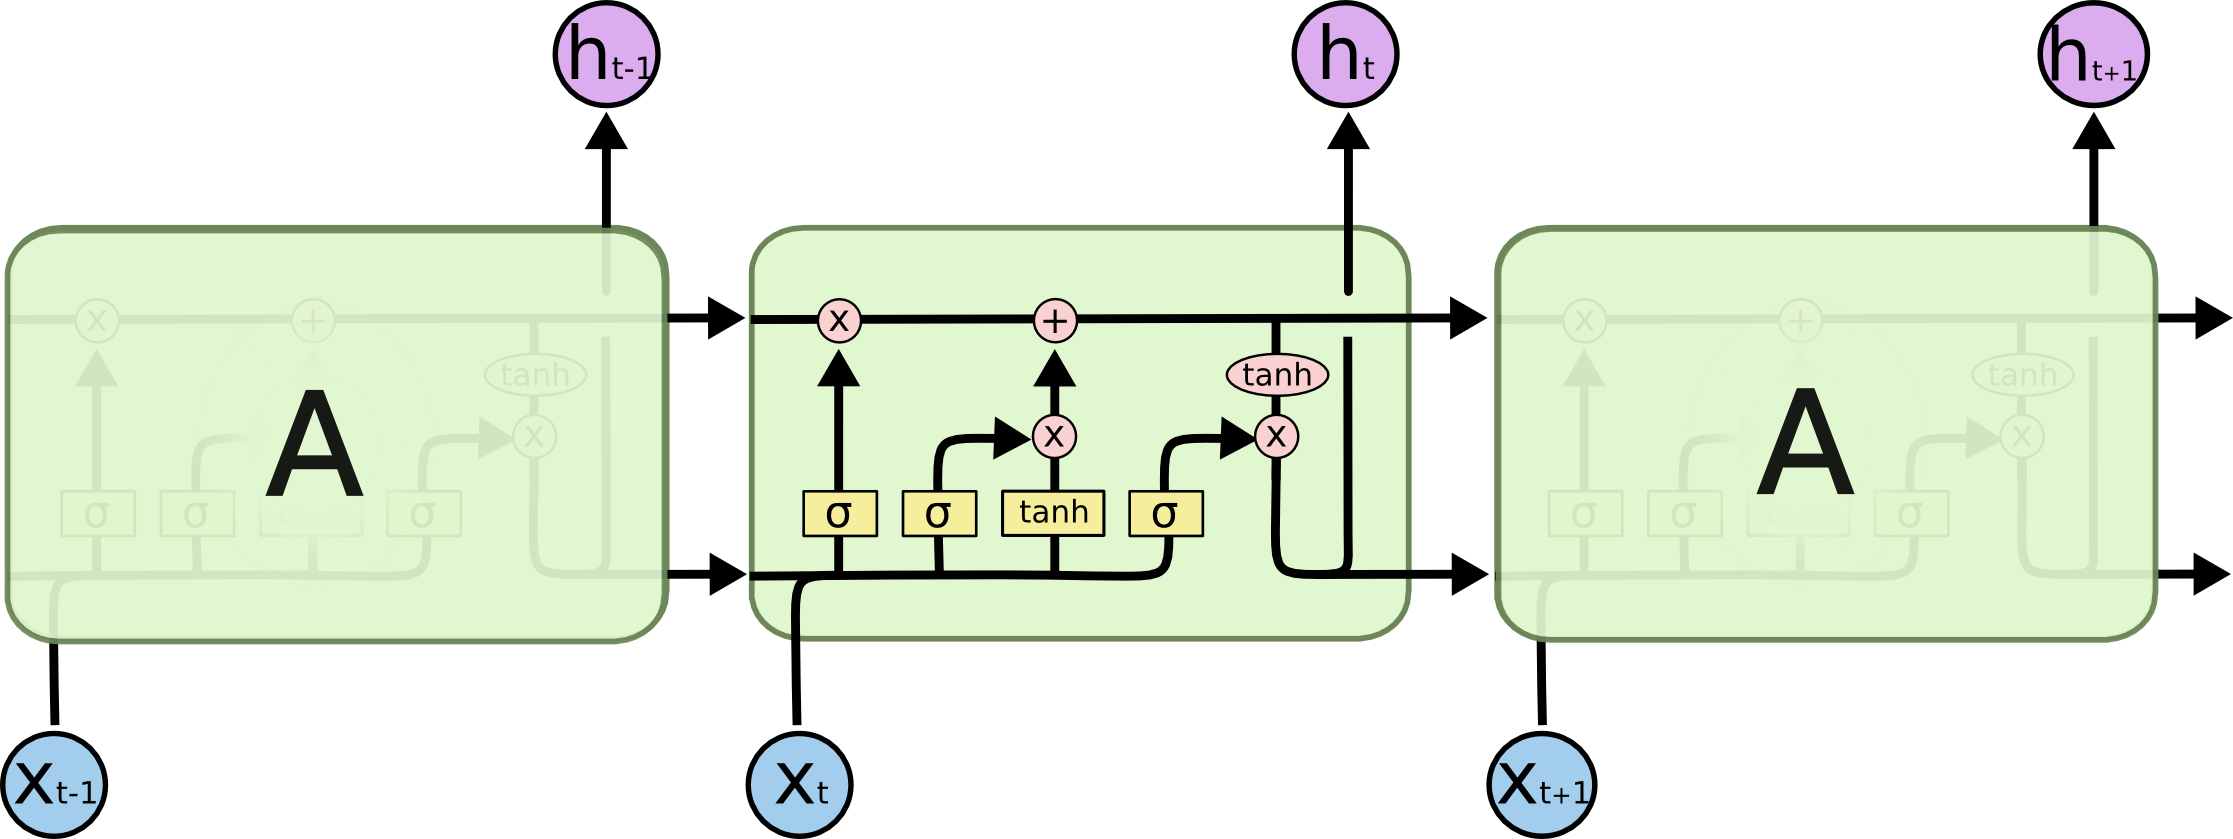
\includegraphics[scale=0.35]{LSTM3-chain.png}
\caption{ساختار شبکه‌های حافظه‌ی طولانی مدت}
\label{fig:lstmf}
\end{figure}

ایده اصلی شبکه های LSTM درواقع داده به نام cell state ها هستند که در تمام طول زنجیره جریان دارند که با هر ماژول در واقع تعاملی خطی و بسیار کم دارند. برای اطلاعات بسیار ساده است که در کنار این داده حرکت کنند و تغییری نداشته باشند. شبکه‌های LSTM توانایی این را دارند که داده از cell state کم کنند یا به آن اضافه کنند که این تغییرات از طریق عملگر‌های ساده‌ای به نام دروازه‌ها (Gate) مانند آنچه در شکل \ref{fig:gate} نشان داده شده اتفاق می‌افتد.
گیت‌ها راهی هستند که داده به صورت انتخابی تغییر بکند یا نکند. این گیت‌ها از یک شبکه عصبی با ساختار sigmoid و یک ضرب نقطه به نقطه تشکیل شده اند.

\begin{figure}[h]
\centering
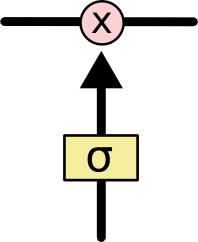
\includegraphics[scale=0.7]{LSTM3-gate.png}
\caption{ساختار ساده‌ی یک گیت}
\label{fig:gate}
\end{figure}

شبکه‌ی عصبی تصمیم میگیرد از هر قسمت چقدر باید عبور کند که صفر یعنی چیزی عبور نکند و یک یعنی تمام مقادیر عبور کنند شبکه‌ی LSTM سه عدد ازین گیت ها دارد که هر کدام تصمیم گیرنده‌ی بخشی از کار هستند. مقدار گیت‌های LSTM در فرمول های \eqref{eq:at} و \eqref{eq:it} و \eqref{eq:ft} و \eqref{eq:ot} مشخص شده‌اند.


\begin{equation}
a^t = \tanh(W_cx^t + U_ch^{t-1}) = \tanh(\hat{a}^t)\label{eq:at}
\end{equation}  

\begin{equation}
i^t = \sigma(W_ix^t + U_ih^{t-1}) = \sigma(\hat{i}^t)\label{eq:it}
\end{equation}  

\begin{equation}
f^t = \sigma(W_fx^t + U_fh^{t-1}) = \sigma(\hat{f}^t)\label{eq:ft}
\end{equation}  

\begin{equation}
o^t = \sigma(W_ox^t + U_oh^{t-1}) = \sigma(\hat{o}^t)\label{eq:ot}
\end{equation}  


\قسمت{تعاریف}\برچسب{chap:not}
در کسب و کار‌ها فرآیند هایی وجود دارند که هدف آن‌ها رساندن سود به مشتری و تولید ارزش می‌باشد. هر فرآیند در واقع تشکیل شده از چند مرحله است که ممکن است در اجرا‌های متفاوت آن دارای مرحله‌ی های متفاوتی باشد. اجرای هر مرحله باعث ثبت یک رخداد در سیستم خواهد شد. 
به زبان ریاضی یک رخداد $e$ یک را می‌توان به صورت $e = (a,c,\tau,D)$ نشان داد که $a \in \mathcal{A}$ در واقع نام مرحله ای است که این رخداد به آن مربوط می‌شود.
همچنین $c \in \mathcal{C}$ در واقع نشان دهنده‌ی آن فرایند به خصوص می‌باشد. $\tau \in T$ نیز نشانگر زمان اجرای این رخداد است. $D \equiv \{(d_1, v_1), \dots, (d_m, v_m)\}$ هم داده‌های اضافه‌ای است که سیستم در اختیار ما برای هر رویداد قرار می‌دهد. 
همچنین عملگر‌های $\pi_{\mathcal{A}}(e) = a$, $\pi_{\mathcal{C}}(e) = c$, $\pi_T(e) = \tau$, and $\pi_{d_i}(e) = v_i$ را نیز بر روی رخداد‌ها تعریف می‌کنیم. یک دنباله به صورت $t = \langle e_1,\ldots,e_n \rangle$ تعریف می‌شود که $\forall \: 1 \leq i \leq |t|, \pi_\mathcal{C}(e_i) = c$.
برای پیشوند و پسوند هم عملگر‌های زیر را تعریف می‌کنیم.

\begin{equation}
t &= \langle e_1, \ldots, e_k,e_{k+1}, \ldots, e_n\rangle \\
\end{equation}
\begin{equation}
\textit{hd}^k(t) &= \langle e_1, \ldots, e_k\rangle\\
\end{equation}
\begin{equation}
\textit{tail}^k(t) &= \langle e_{n-k+1}, e_{n-k+2}, \ldots, e_n\rangle
\end{equation}




\قسمت{روش پیشنهادی}\برچسب{chap:proposal}
در \autoref{chap:not} دنباله‌ها را تعریف کردیم که درواقع دقیقا همان شکل ورودی ای هستند که یک شبکه LSTM از ما انتظار دارد. همچنین در بعضی از سیستم‌های مدیریت فرآیند، داده‌های دیگری برای ما آماده می‌شود که می‌تواند بسیار به دقیق‌تر کردن مدل ما کمک کند. ما فرض می‌کنیم که چنین داده‌هایی می‌توانند در یک بردار سایز ثابت مدل شوند. یک مجموعه از دنباله‌ها که به ما داده شده است باید بتوانیم جوری آن‌ها را مدل کنیم تا برای دادن به شبکه LSTM متناسب باشد.
شبکه‌ی LSTM از ما انتظار دارد که برای ورودی به آن دنباله‌ای از بردار‌های سایز برابر داشته باشیم. برای این مرحله‌ی مربوط به هر رخداد ($\pi_\mathcal{A}(e)$) را با استفاده از روش \lr{one-hot encoding} به صورت بردار در می‌‌آوریم. همچنین برای هر رخداد ویژگی‌های دیگری را نیز استخراج می‌کنیم. این ویژگی‌ها عبارتند از زمان شروع رخداد نسبت به زمان شروع کل فرآیند. زمان شروع رخداد نسبت به اولین روز هفته جاری، زمان شروع رخداد نسبت به رخداد قبلی و زمان شروع رخداد نسبت به اول روز جاری. همچنین برای مدل کردن داده‌های اضافی داده شده می‌توانیم اینگونه عمل کنیم که فرض کنیم تابعی داریم $\textit{count}_{|d_i|}(L)$ که تعداد مقادیر متفاوتی که $d_i$ می‌تواند داشته باشد را به ما برمی‌گرداند که اگر $d_i$ مقداری پیوسته باشد این مقدار عدد 1 می‌باشد. سپس برداری به نام a با طول $\sum_{i=0}^{m} {count}_{|d_i|}(L)$ تعریف می‌کنیم که نمایش برداری ما برای این داده‌ها می‌باشد. برای هر $d_i$، اگر مقداری پیوسته باشد $a[\sum_{j=0}^{i-1}{count}_{|d_j|}(L)]=v_i$ و اگر مقداری کیفی باشد $a[\sum_{j=0}^{i-1}{count}_{|d_j|}(L)+h^i(v_i)]=1$. حال ما برای هر رخداد یک برداد علاوه بر بردار‌های زمانی گفته شده داریم که اندازه‌ی آن به دیتاست ما برمی‌گردد. 
برای فرآیند آموزش شبکه هر ورودی ساخته شده را مساوی دو خروجی قرار می‌دهیم. یکی نمایش one-hot مرحله‌ی بعدی و دیگری زمان رخداد رویداد بعدی که بتوانیم همین داده‌ها را بعد از آموزش پیش‌بینی کنیم.
برای ساختار شبکه عصبی هم از ساختاری مانند \ref{fig:arch}  استفاده کردیم. 
برای بهینه‌سازی پیش‌بینی زمان رخداد بعدی از  MAE و برای پیش‌بینی رخداد بعدی از cross-entropy استفاده میکنیم.
حال که می‌توانیم زمان‌ اجرای مرحله‌ی پس از هر مرحله را پیش‌بینی کنیم. برای یافتن گلوگاه به اینصورت عمل میکنیم که وقتی به ما یک فرآیند ناتمام به عنوان ورودی داده شود، آنقدر عمل پیش‌بینی گام بعدی را تکرار می‌کنیم تا به مرحله نهایی برسیم. سپس ماکسیمم زمان بین مراحل همان گلوگاه است.



\begin{figure}[h]
\centering
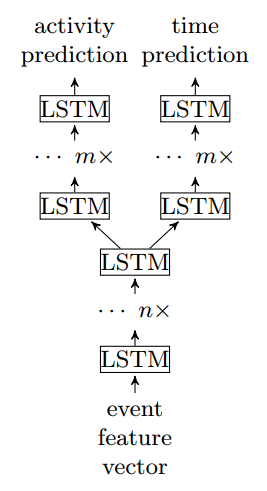
\includegraphics[scale=0.5]{arch.png}
\caption{ساختار شبکه پیشنهادی}
\label{fig:arch}
\end{figure}




\قسمت{داده‌ها}\برچسب{chap:dataset}

برای داده‌های این این پروژه سعی کردیم تا حد امکان از داده‌های واقعی استفاده کنیم. اما برای ساده‌تر کردن پیاده سازی فقط فرآیند‌هایی را نگه داشتیم که به یک مرحله‌ی خاص ختم می‌شوند. داده‌های استفاده شده به صورت زیر هستند. \\
\lr{\textbf{Helpdesk 2017}} \hspace{1cm} این داده مربوط به بخش پشتیبانی و ticketing یک شرکت ایتالیایی به نام SIAV می‌باشد که فعال در حوزه‌ی محتواست.
این داده که در سال 2017 جمع‌آوری شده است، دارای ۱۵۶۸۲ رخداد و ۴۴۵۴ مورد اجرایی و ۱۰ مرحله می‌باشد که دارای ۷ ویژگی علاوه بر زمان رخداد است. که در هر سطر خواص شدت، نوع سرویس‌دهی، درجه سرویس و سختی درخواست وجود دارد. \\

\lr{\textbf{BPI12}} \hspace{1cm} این داده از مسابقه‌ای به همین نام گرفته شده است که در واقع داده‌های یک شرکت مالی فنلاندی می‌باشد. این داده اطلاعات مربوط به فرآیند وام‌گیری افراد در آن وجود دارد. از این داده‌ها، آن قسمتی که دارای نشان "کامل شده" هستند را جدا کردیم و پردازش را فقط بر روی آن‌ها انجام خواهیم داد. این داده دارای در هر سطر دارای مقادیر وام درخواستی و نوع عملیات می‌باشد. مقدار وام درخواستی در کل یک فرآیند ثابت است زیرا مقدار وام درخواستی افراد تغییر نمی‌کند و نوع عملیات می‌تواند شصت نوع مقدار بپذیرد.\\

\lr{\textbf{BPI12\_oneEndAct}} \hspace{1cm} این داده درواقع فیلتر شده‌ی داده‌ی قبلی است. به اینصورت که از آن‌ها، آن فرآیند هایی که به مرحله "\lr{W\_Valideren aanvraag-COMPLETE}" ختم می‌شوند را انتخاب کردیم. به این دلیل که تعداد زیاد از آن‌ها به این مرحله ختم می‌شوند.


\قسمت{جزییات پیاده‌سازی}\برچسب{chap:results}

در این بخش پیاده‌سازی خود را با دو پیاده سازی دیگر یعنی \cite{dats} DATS  و  \cite{process} LSTM مقایسه می‌کنیم.
قابل توجه است که یافتن گلوگاه، همان مساله‌ی پیش‌بینی زمان است، برای همین فقط زمان‌های پیش‌بینی شده در هر پیاده سازی مقایسه شده است.
برای پیاده سازی از چهارچوب نرم‌افزاری \پانویس{Framework}
 Keras استفاده کردیم. تعداد لایه‌های متفاوت و تعداد نورون در هر لایه را برای مقادیر مختلف آزمایش کردیم. تعداد نورون‌های هر لایه را مقادیر ۱۰۰ و ۱۵۰ و ۲۰۰ و ۲۵۰ قرار دادیم و لایه‌ها را به ازای اعداد ۱ تا ۶ آزمایش کردیم. قابل ذکر است که به ازای ساختمان‌‌های متفاوت برای شبکه‌ی عصبی، نتایج تفاوت‌های چندانی نمی‌کنند(تقریبا ۰٫۰۲۵٪ اختلاف در میانگین خطا بین بهترین و بدترین نتیجه). برای الگوریتم یادگیری نیز از Nadam استفاده کردیم. 



\قسمت{سنجش}\برچسب{chap:results}

یک مساله‌ای که وجود دارد این است که یه ازای هر مرحله پیش‌بینی کنیم که مرحله‌ی بعدی که شروع خواهد شد. گفتیمیکیک مساله‌ای که وجود دارد این است که یه ازای هر مرحله پیش‌بینی کنیم که مرحله‌ی بعدی که شروع خواهد شد. گفتیم که دیتاست‌های مورد استفاده‌ی ما فقط دارای فرآیندهایی هستند که تا مرحله‌ی نهایی رفتند. ما از این فرآیندها که به صورت $t = \langle e_1,\ldots,e_n \rangle$ نمایش مي‌دهیم و دارای طول n هستند، تمام دنباله‌های پیشوندی به طول $1\leq k \leq n-1$ را می‌سازیم و به عنوان ورودی به شبکه ‌خود می‌دهیم. از هر داده حدود 2/3  آن را برای آموزش و اعتبارسنجی مدل خود استفاده می‌کنیم. خروجی این آموزش درواقع ساختار و وزن‌های شبکه‌ی عصبی ماست. همچنین از 1/3 داده‌ی باقی‌مانده برای ارزیابی مدل استفاده می‌کنیم. 
برای ارزیابی مدل خود از معیار میانگین خطای مثبت  \پانویس{MAE} استفاده میکنیم. فرض کنیم که $y_i$ مقدار پیش‌بینی شده باشد و $\hat{y_i}$ مقدار واقعی روی مدل با ورودی $x_i$ به ازای $\{x_i | 0\leq i\leq n\}$ باشد. این معیار را طبق فرمول \eqref{eq:mae}  تعریف میکنیم.
\begin{equation}
MAE=\frac{\sum_{i=0}^n |y_i - \hat{y_i}|}{n}. \label{eq:mae}
\end{equation}

\begin{table}[t]
    \centering
    \begin{latin}
    \begin{tabular}{|l|c|c|c|}
    \hline
   Method/Dataset & Helpdesk2017 & BPI12 & BPI12\_oneEndAct \\
    \hline
    DATS  & 5.27  & 8.13 &5.44\\
   % CONTEXT-SVR-SEQ~\cite{Polato2014}  & 4.34 & & & 8.76* & 5.85*\\
  %  CONTEXT-SVR-SET~\cite{Polato2014} & 15.68 & 4.40 & & & 8.03 & 5.36 \\
  %  CONTEXT-SVR-BAG~\cite{Polato2014} & 15.69 & 4.42 & & & 8.29* & 5.54*\\
 % LSTM~\cite{Tax2017} & 4.03  &9.74~ &5.95~ \\
    LSTM & 4.03  &9.74~ &5.95~ \\
      & (n=150, l=5)  &(n=150, l=5) &(n=100, l=3) \\

%      & (n=150, l=5)  &(n=100, l=3) &(n=100, l=3) \\
\hline
   Our Proposal  &\textbf{4.01} & \textbf{7.04}& \textbf{4.65} \\
    & (n=250, l=5) &(n=100, l=4) &(n=250, l=1) \\
   \hline
    \end{tabular}
    \end{latin}

    \caption{مقایسه‌ی پیاده سازی های مختلف. اعداد بیان شده به روز هسنند.}
    \label{tab:results}
\end{table}

در جدول \ref{tab:results} نتایج سنجش‌های ما گزارش شده است. همچنین ساختار شبکه نیز در این گزارش توصیف شده است. میبینیم که با داده‌های HELPDESK پیاده سازی ما و cite{process} LSTM\ تقریبا نتایج یکسانی را گزارش می‌دهند. با بررسی داده‌های موجود در BPI12 متوجه خواهیم شد که یک مرحله ممکن است حاوی چند رخداد باشد و این در پیاده‌سازی \cite{process} LSTM مشکل‌ساز خواهد شد. در داده‌های ‌HELPDESK بیشتر اطلاعات داخل روند انجام مراحل نهفته است و نه داخل داده‌های اضافی داده شده است ولی در BPI12 بیشتر اطلاعات از داده‌های اضافی استخراج می‌شود. به همین علت است که می‌بینیم  \cite{process} LSTM جواب خوبی به ما نمی‌دهد.

\فصل{جمع‌بندی و گام بعدی}\برچسب{chap:conclusion}

در این پروژه نتایج مقالات مختلف را بررسی کردیم و به راه حلی برای یافتن گلوگاه در فرآیندهای کسب و کاری رسیدیم که می‌توان از این گلوگاه‌ها برای مدیریت منابع بهتر استفاده کرد. برای بهتر کردن این نتایج ایده‌های متفاوتی مطرح می‌شوند. یکی از مشکلاتی که در این مدل وجود دارد سایز بزرگ بردار‌های ساخته شده از روی داده‌های اضافی تهیه شده است که روند آموزش مدل را کند و نادقیق می‌کند همچنین مقدار حافظه‌ی مصرف شده را زیاد می‌کند. می‌توان برای بهبود حافظه از روش‌های کدسازی \پانویس{hashing} بهینه استفاده کرد. برای بهتر کردن مدل خود می‌توانیم از گیت‌های تازه معرفی شده‌ی GRU به جای LSTM استفاده کنیم و نتایج حاصل را مقایسه کنیم. همچنین می‌توان دیگر رویکرد‌های یادگیری ماشین را نیز برای این مساله به کار برد. به عنوان مثال از روش‌های SVM مبتنی بر دنباله‌ها استفاده کنیم.


\PrepareForBiblio
\begin{thebibliography}{1}
\begin{LTRitems}
\setpersianfont
\bibitem{data-aware}\resetlatinfont
\newblock {\itshape LSTM Networks for Data-Aware Remaining Time Prediction of Business Process Instances}.
Nicolò Navarin, Beatrice Vincenzi, Mirko Polato, Alessandro Sperduti
\setpersianfont
\bibitem{process}\resetlatinfont
\newblock {\itshape Predictive Business Process Monitoring with LSTM Neural Networks}. 
Niek Tax, Ilya Verenich, Marcello La Rosa, Marlon Dumas
\setpersianfont
\bibitem{datawarehouse}\resetlatinfont
\newblock {\itshape Beyond Data Warehousing : What’ s Next in Business Intelligence ? In 7th ACM international workshop on Data warehousing and OLAP, pages 1–6, 2004.}
M. Golfarelli, S. Rizzi, and I. Cella
\setpersianfont
\bibitem{regression}\resetlatinfont
\newblock {\itshape time prediction: When will this case finally be finished? Lecture Notes in Computer Science (including subseries Lecture Notes in Artificial Intelligence and Lecture Notes in Bioinformatics), 5331 LNCS (PART1):319–336, 2008}
B. F. Van Dongen, R. A. Crooy, and W. M. P. Van Der Aalst.
\setpersianfont
\bibitem{next}\resetlatinfont
\newblock {\itshape Supporting flexible processes through recommendations based on history. In Proceedings of 6th International Conference BPM, pages 51–66. Springer, 2008.}
H. Schonenberg, B. Weber, B. F. van Dongen, and W. M. P. van der Aalst.

\setpersianfont
\bibitem{tree}\resetlatinfont
\newblock {\itshape Completion time and next activity prediction of processes using sequential pattern mining. In Discovery Science - 17th International Conference, DS 2014, Bled, Slovenia, October 8-10, 2014. Proceedings, pages 49–61, 2014.}
M. Ceci, P. F. Lanotte, F. Fumarola, D. P. Cavallo, and D. Malerba.

\setpersianfont
\bibitem{deep1}\resetlatinfont
\newblock {\itshape A Deep Learning Approach for Predicting Process Behaviour at Runtime, pages 327–338. Springer International Publishing, Cham, 2017.}
J. Evermann, J.-R. Rehse, and P. Fettke.

\setpersianfont
\bibitem{cluster1}\resetlatinfont
\newblock {\itshape  Complex symbolic sequence clustering and multiple classifiers for predictive process monitoring. In 11th International Workshop on Business Process Intelligence 2015, pages 218–229, Innsbruck, Austria, December 2016. Springer}
I. Verenich, M. Dumas, M. L. Rosa, F. M. Maggi, and C. D. Francescomarino.

\setpersianfont
\bibitem{dats}\resetlatinfont
\newblock {\itshape  Data-aware remaining time prediction of business process instances. In 2014 International Joint Conference on Neural Networks (IJCNN), pages 816–823. IEEE, jul 2014.}
M. Polato, A. Sperduti, A. Burattin, and M. de Leoni.
\end{LTRitems}
\end{thebibliography}

\PrepareForLatinPages
\date{February 5, 2020}
\title{\sffamily Finding bottlenecks of business processes using deeplearning methods}
\author{\sffamily Seyed Morteza Hoseini}
\university{Shahid Beheshti University\\Computer Science and Engineering Faculty}
\supervisor{\sffamily Dr. Sadegh Aliakbari}

\makethesistitle

\پایان{نوشتار}